\chapter{Implementering og Test}
\label{ch:Implementering og test af Algoritmerne}

I dette afsnit testes algoritmerne fra afsnit \ref{ch:Sorteringsalgoritmer}. Algoritmerne implementeres i python.

\section{Python}
\label{sec:Python}

Sproget Python har et højt abstraktionsniveau, og kan på mange punkter ligne vores pseudokode fra tidligere \cite[s. 68]{aogd}. Det betyder at vi på mange punkter opgiver lidt kontrol til compileren, for at gøre koden mere læsbar og tilgængelig. Det betyder også at vi aldrig helt kan vide hvilke instruktioner computeren udfører. Derudover er Python et relativt langsomt sprog, da koden kompileres samtidigt med at programmet kører \cite{what-is-python}. Dette gør at sproget ikke egner sig særligt godt til at skrive optimerede algoritmer, der skal køre på meget store datasæt. Heldigvis kan vi se bort fra dette, da vi med store-O-analyse er ligeglade med den reelle udførelsestid, og i stedet er interesseret i vækstrater. Vækstraten for en algoritme er nemlig egns, ligegyldigt hvor langsomt hvert skridt er. På nogle punkter er det måske endda en fordel, at algoritmerne kører langsommere, da det vil gøre forskellen i udførelsestiderne større, og lettere at forholde sig til. 


\section{Implementering}
\label{sec:Implementering}

Implementering i Python er relativt simpelt. Python bruger dynamiske variabler \cite{what-is-python}, derfor er det ikke nødvendigt at fortælle Python, om en variabel f.eks. er et heltal eller en liste. 

%\begin{figure}
	%\begin{center}
		%\lstinputlisting{../python/algoritmer/insertionsort.py}
	%\end{center}
	%\caption{Insertionsort i Python}
	%\label{fig:Insertionsort i Python}
%\end{figure}

\section{Test af Sorteringsalgoritmer}
\label{sec:Test af Sorteringsalgoritmer}

For at teste sorteringsalgoritmerne fra afsnit \ref{ch:Sorteringsalgoritmer}, og se hvordan deres reelle udførelsestid som funktion af $n$, relaterer til deres teoretiske væksthastighed og store-O-analyse, skal algoritmerne køres på en kontroleret måde hvor vi systematisk kan tage tid på algoritmens udførelsestid ved forskellige input.\\

På figur \ref{fig:Kode til test af algoritmerne} på side \pageref{fig:Kode til test af algoritmerne} ses koden til test af algoritmerne. Variablen $functions$ på linje $1$ indeholder en liste med de algoritmer, der skal testes. I vores tilfælde indeholder den $[insertionsort,mergesort]$. Inde i denne løkke tester vi funktionerne. Det at vi behandler algoritmerne ens, sikrer at de bliver testet på samme måde. Det næste vi gør er at definere lister til opbevarting af kardinaliteten af den liste som algoritmen sorterer (l. $4$), og en til den reelle tid det tager for algoritmen at sortere listen (l. 6).  I linje $9$ sætter vi frøet for de pseudotilfældige tal \cite{python-random}, som vi senere skal bruge til at generere listerne som sorteringsalgoritmerne skal sortere. Det er vigtigt af vi sætter frøet til den samme værdi, før vi tester hver algoritme, da vi på den måde sikrer os, at det er de samme pseudotilfældige lister, som algorimerne sorterer. Vi kan derfor med god vilje sammenligne algoritmernes køretider, da vi er sikre på at deres input, var det samme under testen. Efter denne pegerer (l. 12 og 15). Den første sørger for at vi gentager den samme test flere gange. I vores tilfælde er variablen $trials$ sat til $15$, hvilket resulterer i at vi tester sorteringen af hver $n$ lange liste $15$ gange. Den indre løkke tæller fra $i=0$ til $i=80$. Vi bruger herefter $i$-værdien til at generere vores $n$-værdier i linje $18$. Til det bruges formlen $n=\nint{1.1^i}$. Valget at test med exponentielt stigende $n$, er af to grunde: For det første kan det tage lang tid for en algoritme, at sortere lister med store $n$, så det gør hele processen meget hurtigere, hvis man ikke tester så mange sorteringer med store $n$. Den anden og nok bedre grund, er at vi er meget interesserede i at se hvordan algoritmerne måles med hinanden, når $n$ \emph{ikke} er stort. Det ville jo være interessant, hvis vi kunne identificere et $n_0$ som i afsnit \ref{ch:Algoritmers Udførelsestid}. Til dette skal vi bruge en punkttæthed, der ved store $n$ ville være overflødig.\\

Nu er det hele sat op, og vi kan teste algoritmen på en $n$ lang liste med tilfældige tal. $n$-værdien og den tid sorteringen tog, gemmes i listerne, og eksporteres til en csv fil til brug i databehandlingen (se koden i bilag 1 og 2).

\begin{figure}
	\begin{center}
		\lstinputlisting[firstline=53,lastline=81]{../python/sorting.py}
	\end{center}
	\caption{Kode til test af algoritmerne. Variablen $functions$ er en liste med de to algoritmer der testes ([insertionsort,mergesort]).}
	\label{fig:Kode til test af algoritmerne}
\end{figure}



\section{De Reelle Udførelsestider}
\label{sec:De Reelle Køretider}

Algoritmernes udførelsestider er plottet i figur \ref{fig:plot - to algoritmer} på side \pageref{fig:plot - to algoritmer}.\\

Som det tydeligt fremgår på graferne, er mergesort langt hurtigere end insertionsort ved store $n$. Vi kan også se at algoritmerne nogenlunde følger deres regressioner, men hvorfor egentlig det? Det er kun i værste tilfælde at $T_{insertionsort}(n) \in \Theta (n^2)$ ikke? Jo, men det lader til at insertionsorts gennemsnitlige vækstrate, er tættere på $\Theta (n^2)$ end på $\Theta (n)$. Det er dog alligevel tydeligt at andengradsregression ikke passer helt på insertionsorts gennemsnitlige køretid, hvis vi zoomer ind på plottet til højre på figur \ref{fig:plot - to algoritmer}. Faktisk passer regressionen slet ikke på punkterne på dette stykke af grafen, hvilket tyder på at algoritmens udførelsestid ikke bare kan beskrives med et andengradspolynomie. Hvad angår mergesort følger den regressionen rigtig godt. Det tyder på at antagelsen at mergesorts vækstrate altid er $\Theta (n \log n)$ fra afsnit \ref{sec:Mergesort og Den Nedre Grænse} må være sand.\\

En anden finurlighed kan findes i residualplottet (figur \ref{fig:toAlgoritmerResidual}). Residualplottet for begge grafer er rigtig flot, med en jævn punktfordeling på begge sider af regressionen, men til aller sidst er der et par af insertionsorts punkter, der er langt under regressionen. Det kan være af flere grunde blandt andet at computerens styresystem lige i dette tilfælde, tildelte flere ressourcer til programmet. En anden grund kunne være at algoritmen netop i disse tilfælde, var heldig at få en delvist sorteret liste, der gjorde at listen kunne sorteres langt hurtigere end $O(n^2)$. Dog tyder det tydelige nedadgående mønster i outlier-residualerne på, at afvigelsen ikke er en tilfældighed.\\

Når man ser på residualplottene er et andet mønster også tydeligt: variansen stiger. Udførelsestiderne har større og større usikkerhed, jo større $n$ er. Dette giver intuitivt mening hvis man sætter det i kontekst. Hvis $10$ personer løber et $50$m løb, vil alle løbere afslutte inden for et forholdsvist lille tidinterval. Hvis vi herefter bad dem om at løbe et maraton, ville deres tider ikke bare variere med sekunder og minutter, men med timer. Variansen i deres tider, øges altså af størrelsen på opgaven. Det samme er sandt for vores sorteringsalgoritmer, hvilket tydeliggøres af residualplottene. 


\subsection{Hvornår er Insertionsort Hurtigst?}%
\label{sub:Store-O er Værste Tilfælde}
Det er tydeligt at mergesort er langt bedre, til at sortere store lister, men ved små $n$ kan vi også se at insertionsort, ikke er langt bagefter. Faktisk er den \emph{gennemsnitlige} sortering hurtigere eller nogenlunde ens før $n = 37$ (se figur \ref{fig:toAlgoritmerZoomedGns}). Det bekræfter teorien fra afsnit \ref{ch:Algoritmers Udførelsestid}, idet at store-O ikke siger noget om algoritmens opførsel ved små $n$, men kun ved meget store. Her er det tydeligt at en sådan form for analyse ikke er tilstrækkeligt for at bedømme, hvilken algoritme der er bedst til hvilke problemer. Store-O analyse er også blind overfor den gennemsnitlige udførelsestid. Ved små $n$ er den gennemsnitlige køretid brugbar, da den maksimale køretid aldrig bliver astronomisk stor, og vi kan derfor med god vilje bruge gennemsnitlig udførelsestid i disse overvejelser. Det ville gennemsnitligt være hurtigst, at bruge insertionsort, ved små $n$ og mergesort ved store. Punktet der adskiller hvilken algoritme der er hurtigst er ca. $n = 37$. Dette punkt kan siges at svarer til $n_0$ fra afsnit \ref{ch:Algoritmers Udførelsestid}, idet at mergesort gennemsnitligt altid er hurtigere efter punktet. Alligevel er det ikke helt sandt, da $n_0$ fra afsnit \ref{ch:Algoritmers Udførelsestid} forholder sig til værste-tilfælde-udførelsestiden, men vi kan i denne reelle kontekst bruge $n_0$, som punktet hvorefter mergesort \emph{gennemsnitligt} er hurtigst.

%...grunden til at bruge algoritmens gennemsnitlige udførelsestid er...

% mergesort kølrer altid med store Theta(n)


\begin{figure} \centering
	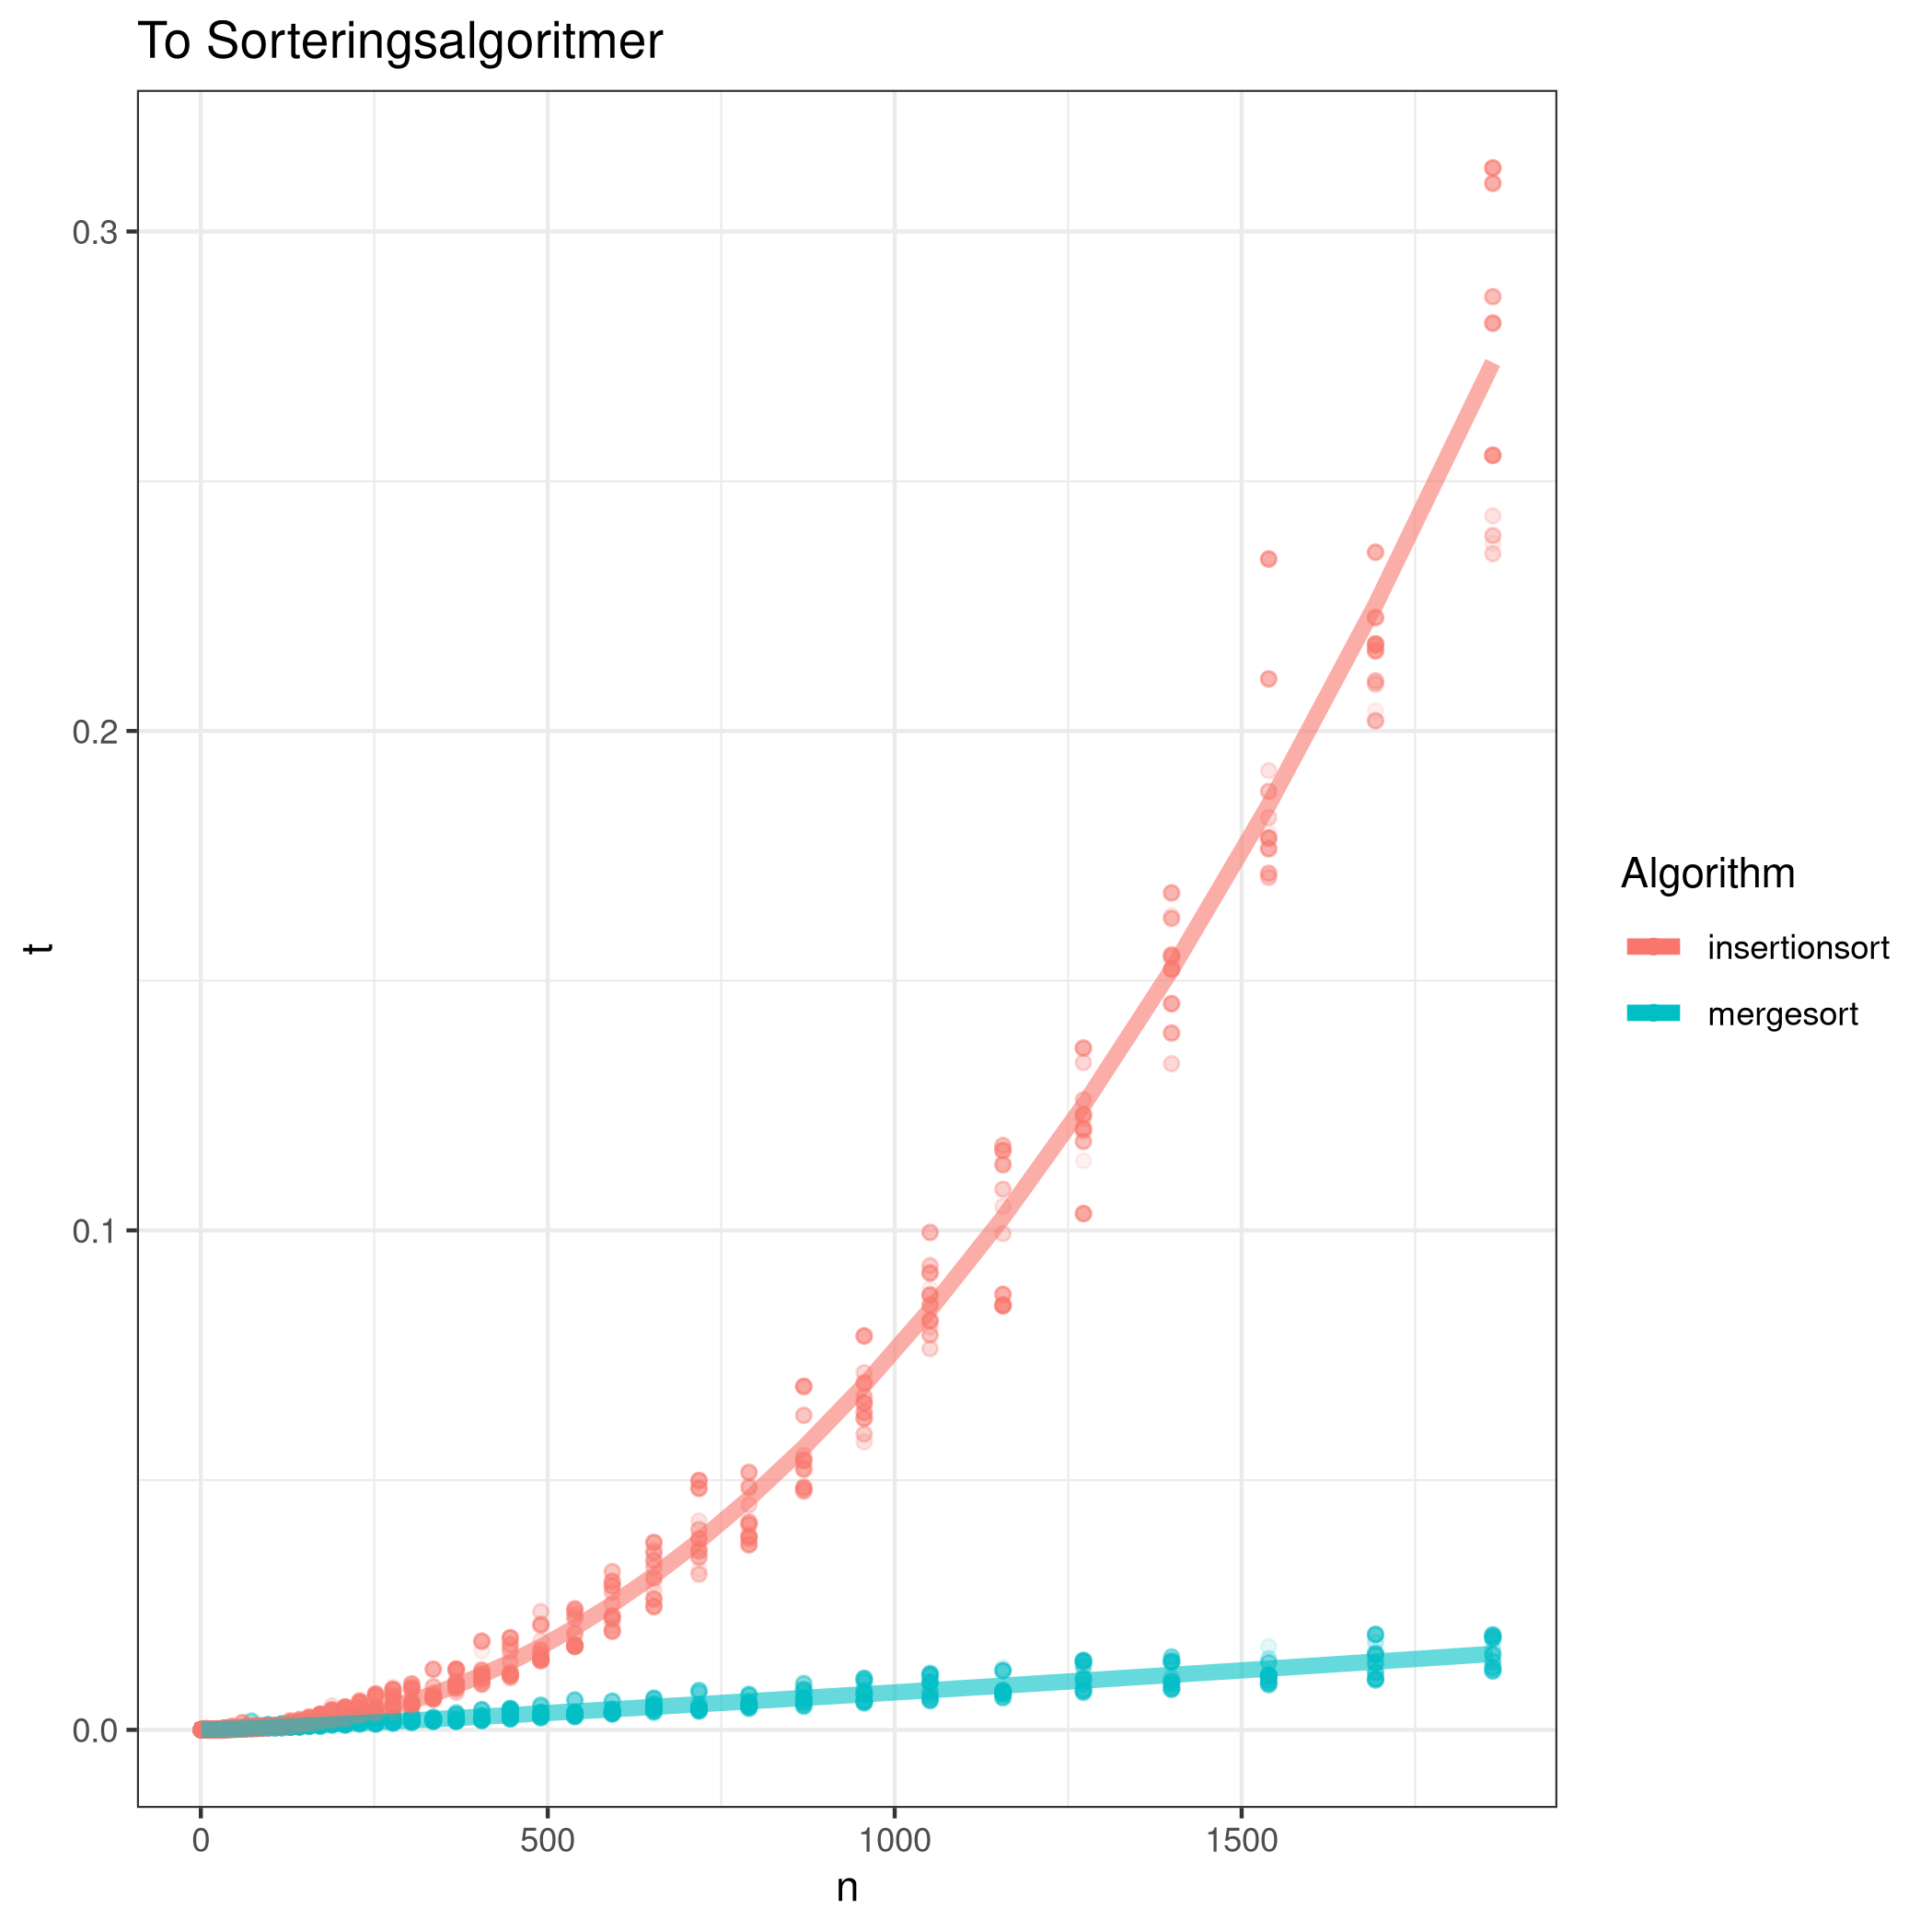
\includegraphics[width=0.45\textwidth]{../img/toAlgoritmer.png}
	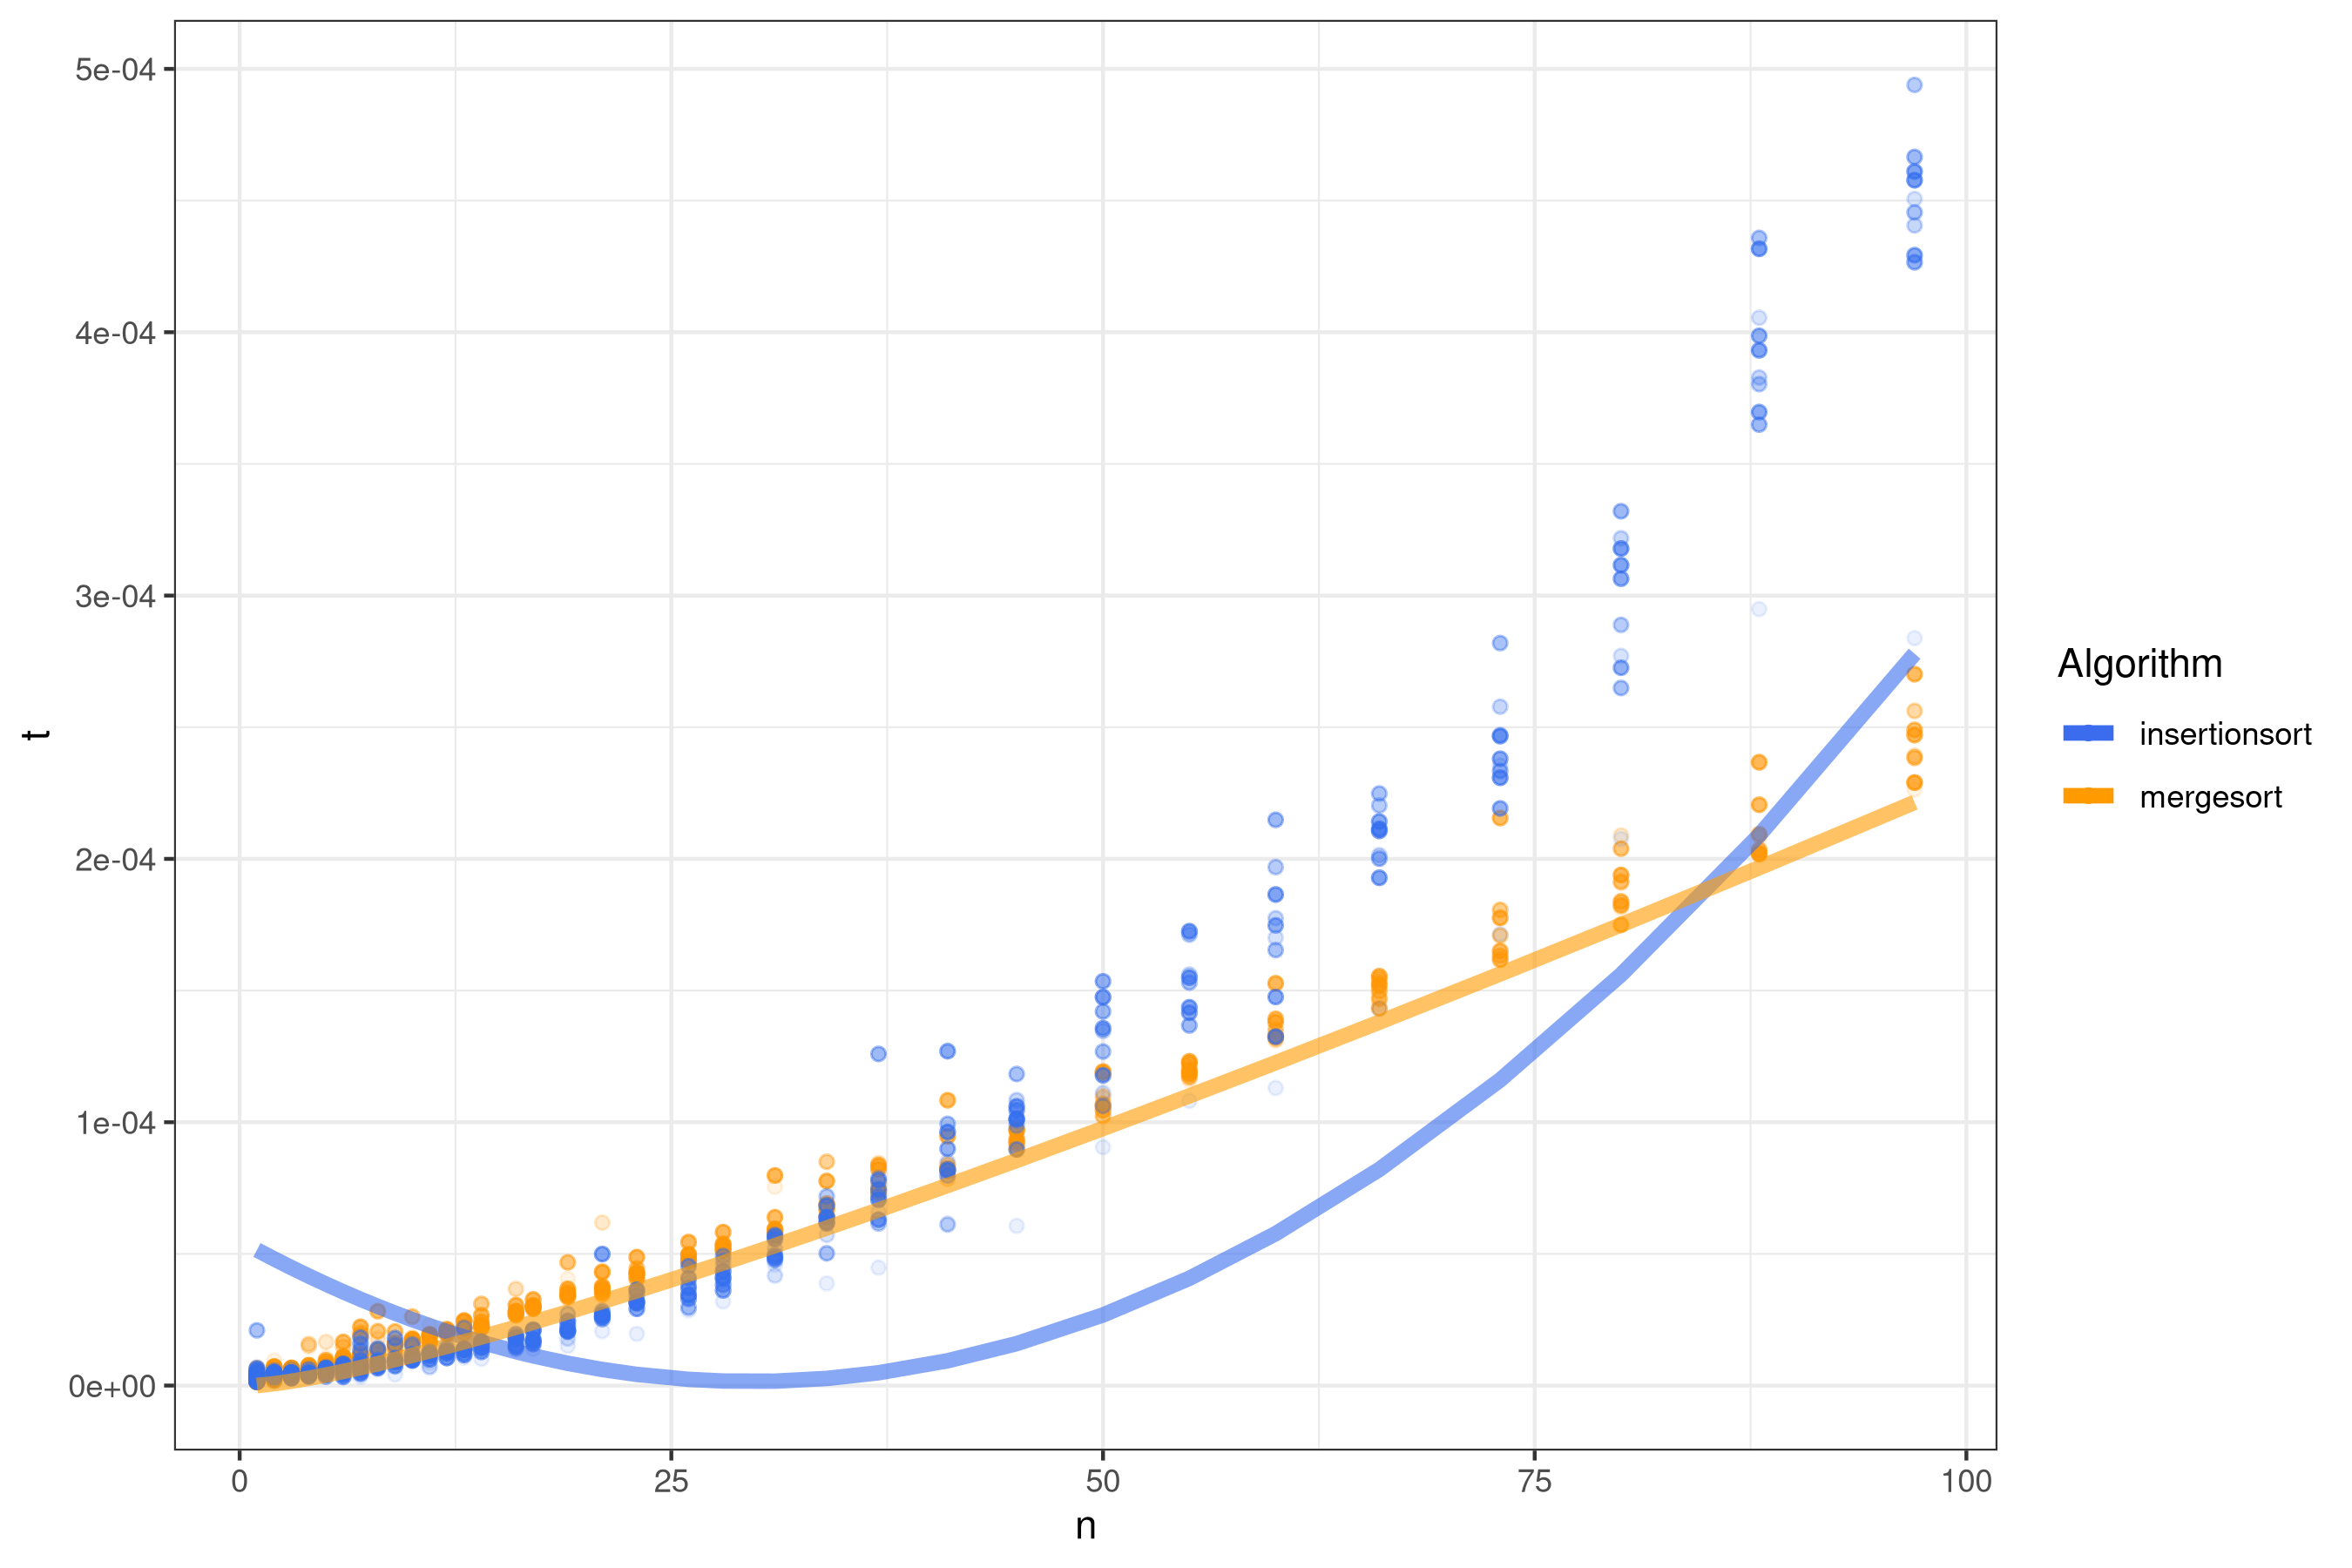
\includegraphics[width=0.45\textwidth]{../img/toAlgoritmerZoomed}
	\caption{Sammenligning af insertionsort og mergesort. Til venstre ses grafen for de to algoritmer sammen med en regression. Regressionerne er henholdsvis en andengradsregression for insertionsort, og en $a \cdot n \cdot \log n$-regression for mergesort.}
	\label{fig:plot - to algoritmer}
\end{figure}

\begin{figure}
	\begin{center}
		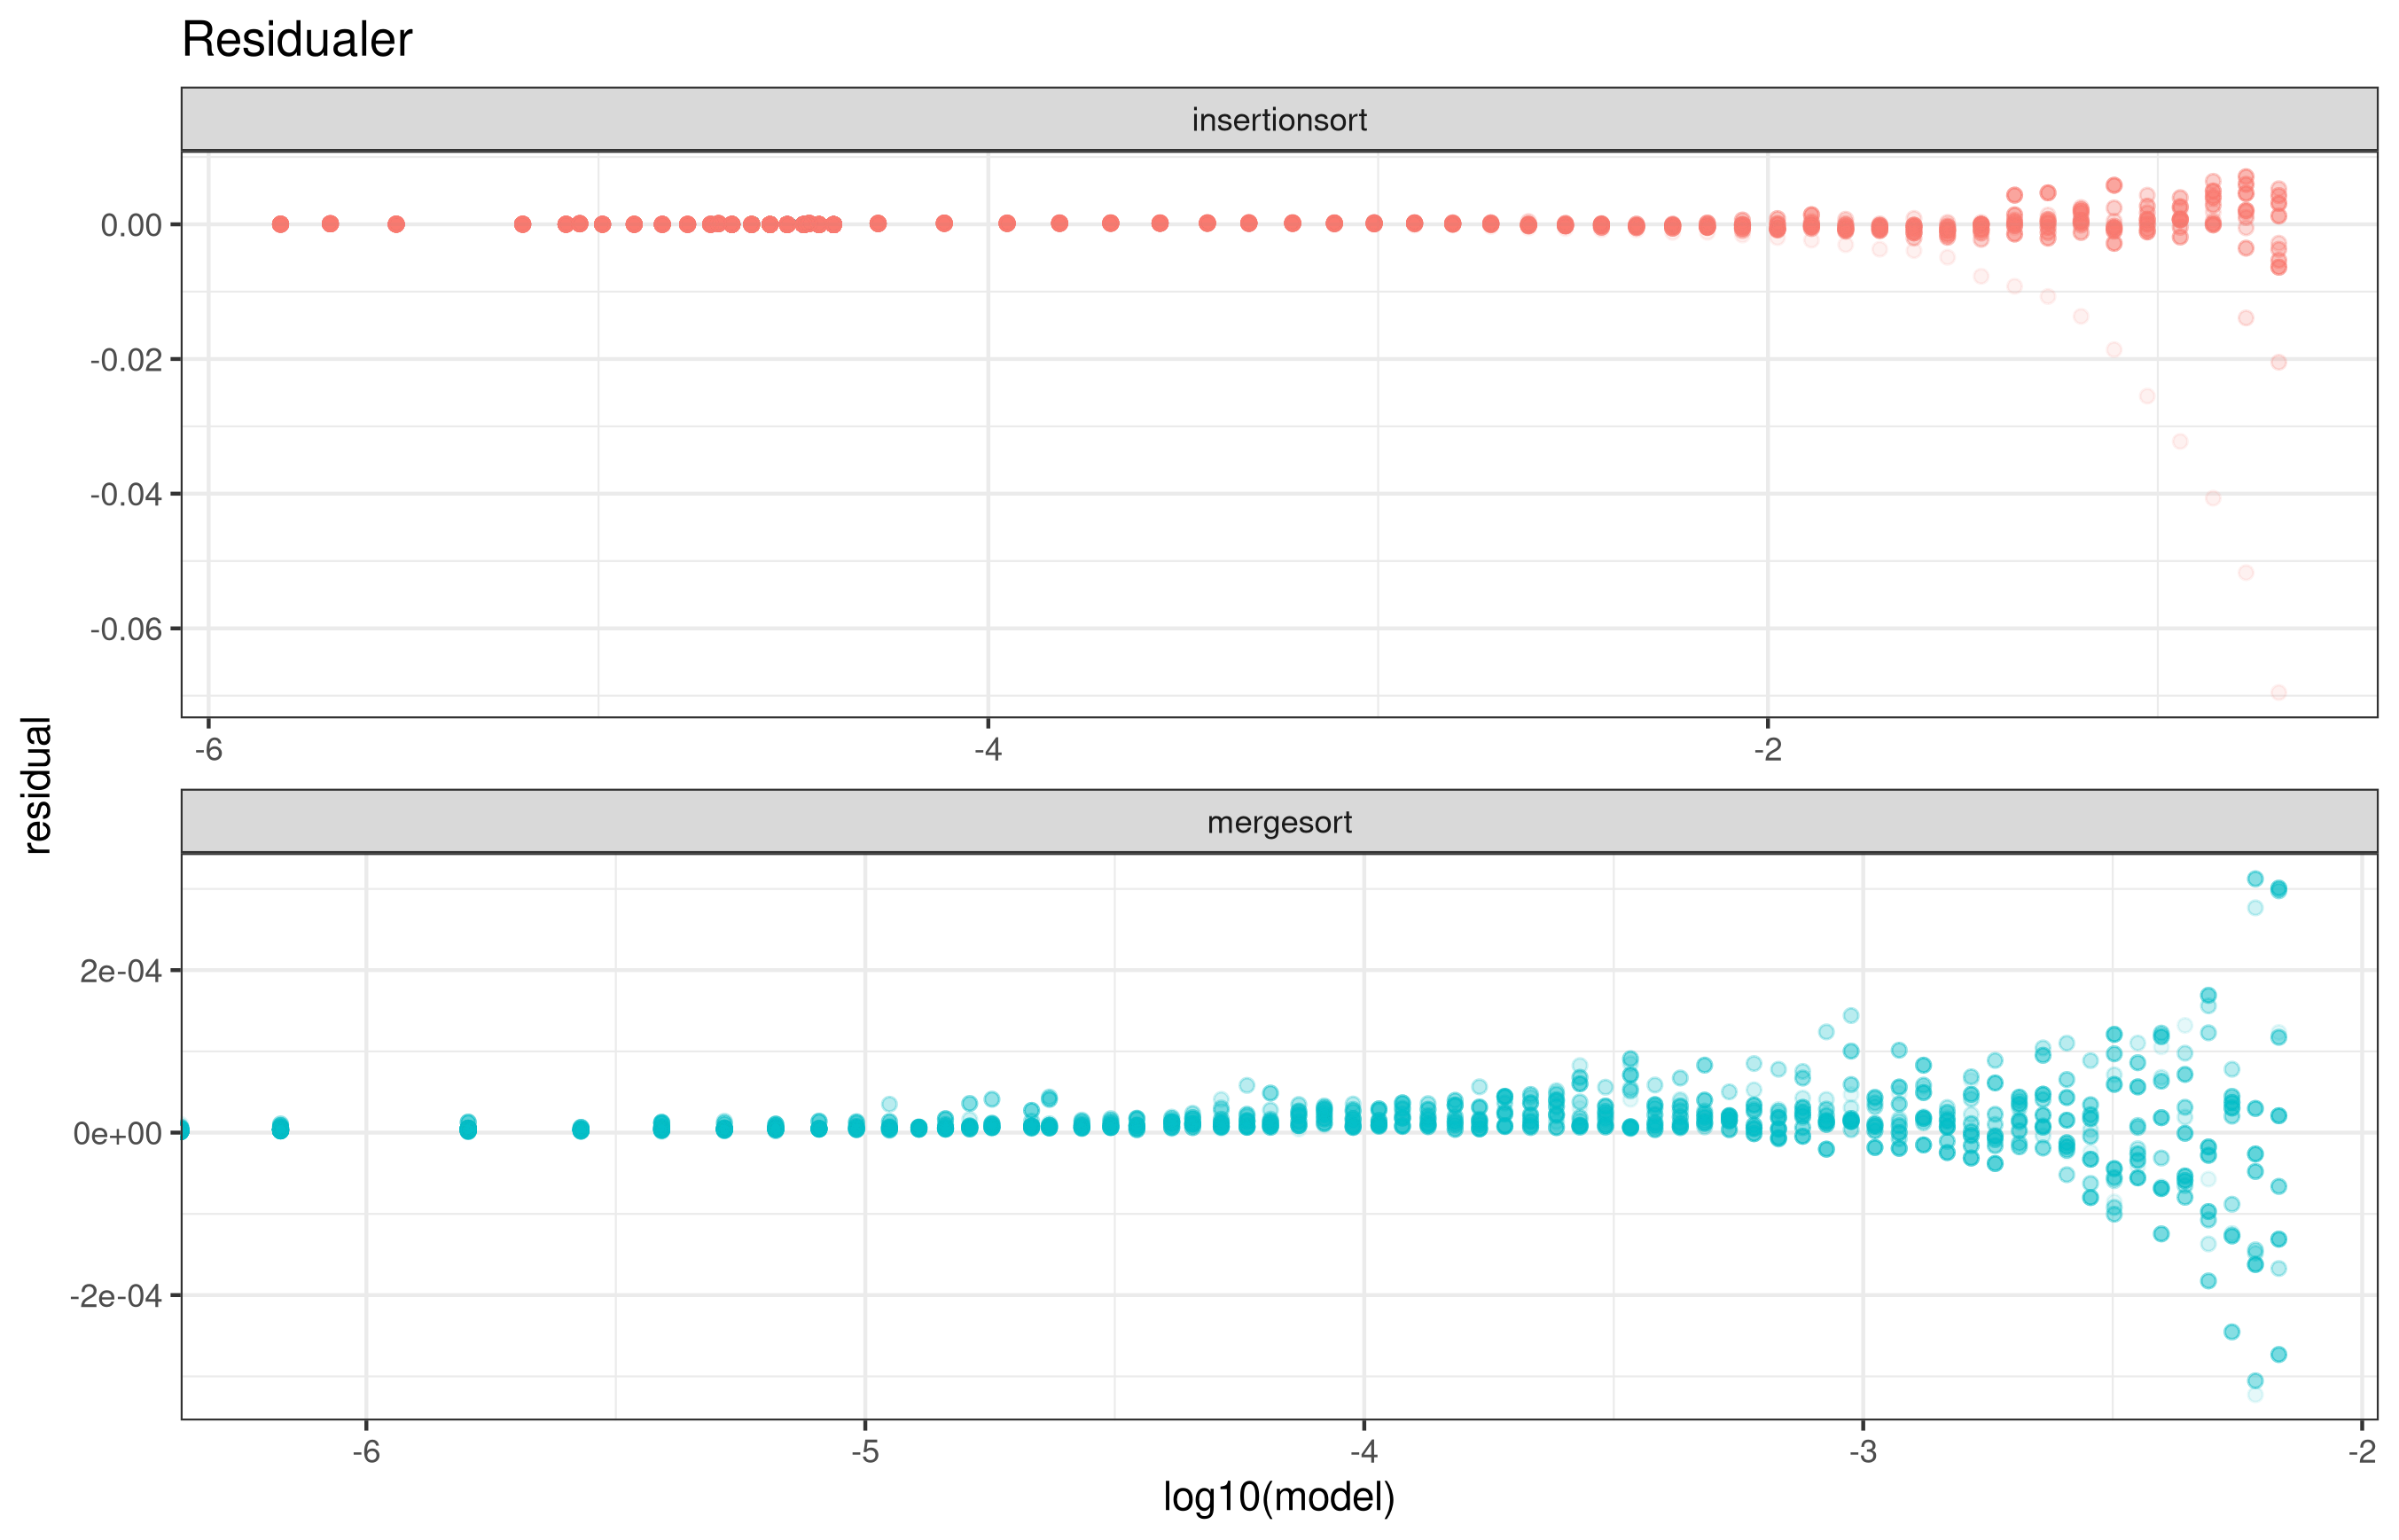
\includegraphics[width=0.75\textwidth]{../img/toAlgoritmerResidual.png}
	\end{center}
	\caption{Residualplot for modellerne i figur \ref{fig:plot - to algoritmer}.}
	\label{fig:toAlgoritmerResidual}
\end{figure}



\begin{figure}
	\begin{center}
		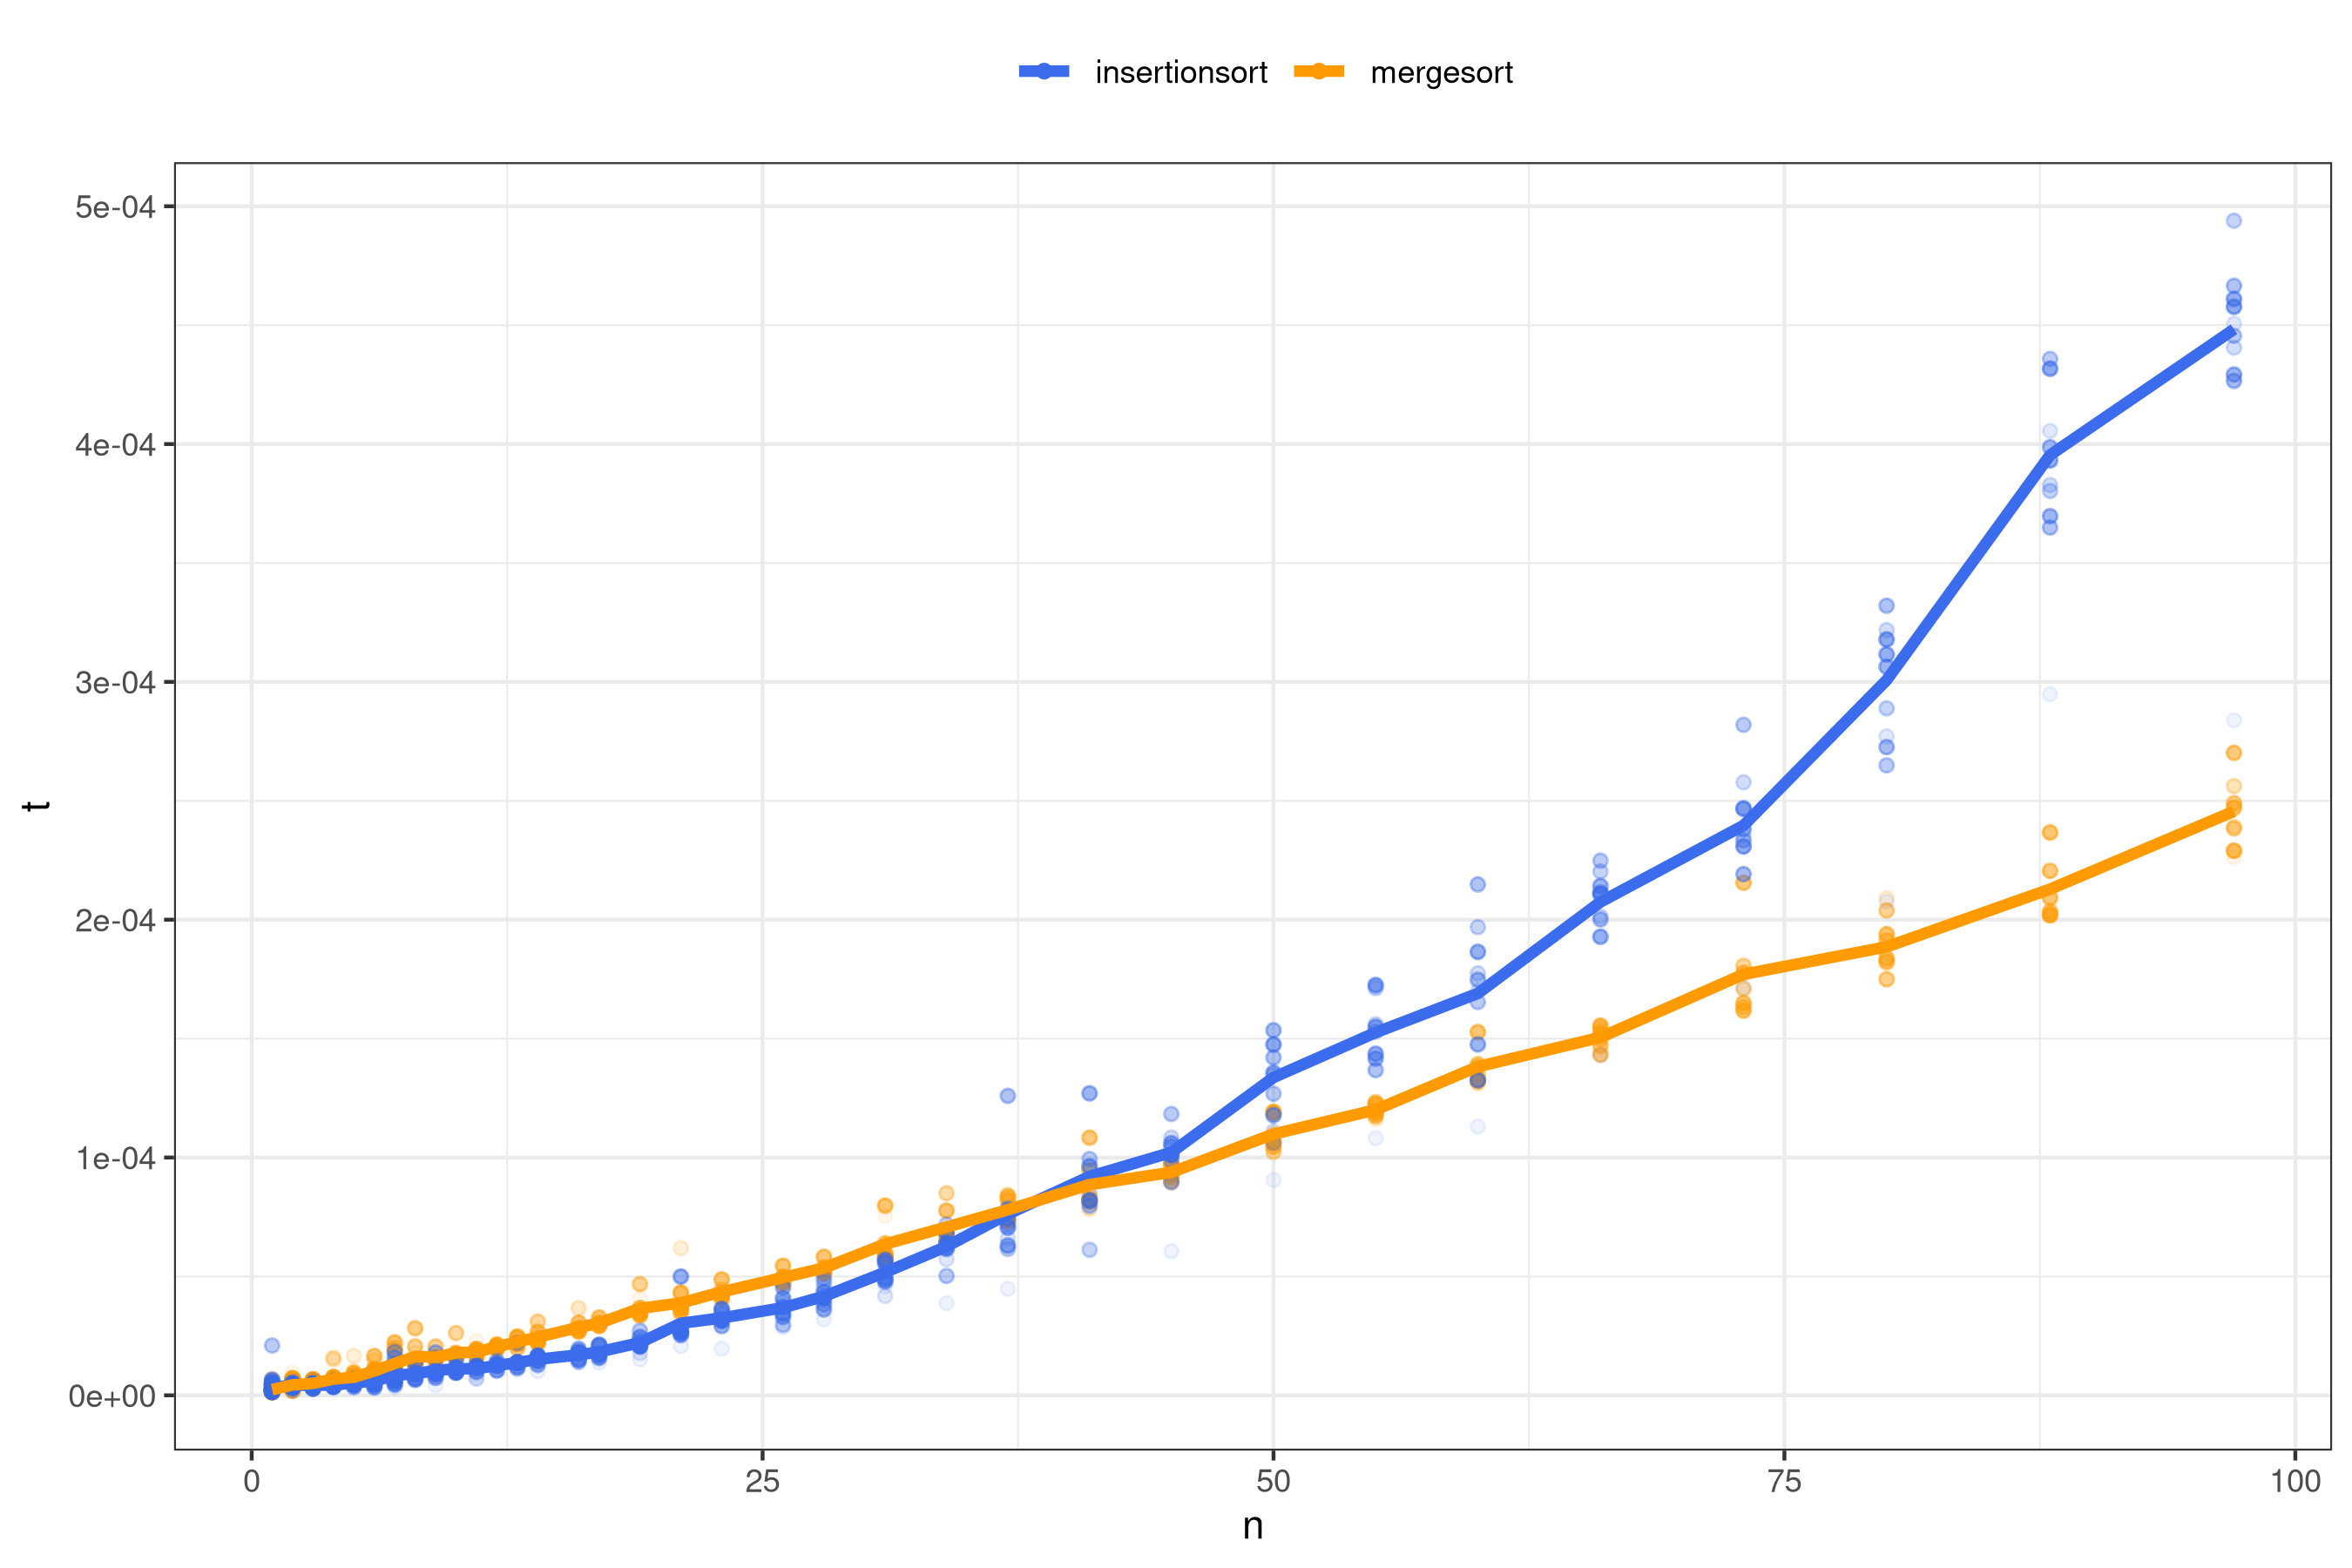
\includegraphics[scale=0.6]{../img/toAlgoritmerZoomedGns.png}
	\end{center}
	\caption{Dette er samme data som i figur \ref{fig:plot - to algoritmer}, men zoomet ind til indervallet $n \leq 100$. Her er regressionerne erstattet af en linje der går mellem gennemsnittet af $t$ for hver $n$. Det interessante ved grafen er, at man tydeligt kan de hvordan insertionsort gennemsnitligt er hurtigst, indtil $n \approx 37$ hvorefter mergesort er hurtigst.}
	\label{fig:toAlgoritmerZoomedGns}
\end{figure}

\section{Optimering af Mergesort}%
\label{sub:Optimering af Mergesort}

At insertionsort faktisk normalt er hurtigere end mergesort hvis $n < n_0$, betyder at den hurtigste måde at sortere en liste afhænger af listens længde: Er listen på under $n_0$ elementer? så brug insertionsort. Er listen over $n_0$ elementer? så er mergesort gennemsnitligt hurtigere. Dette kunne lede os til at lave en ny sorteringsalgoritme således:

\begin{figure}[h]
	\begin{center}
		\begin{lstlisting}
		def sort(liste) {
			if liste.length <= 37 {
				return(insertionsort(liste))
			}
			return(mergesort(liste))
		}
		\end{lstlisting}
	\end{center}
	\vspace{-6mm}
	\caption{Algoritme der bruger insertionsort hvis inputlisten er kortere end $37$, og ellers mergesort.}
	\label{fig:hybridalgoritme}
\end{figure}


Her bruger vi insertionsort hvis listens længde er under eller lig $37$, og mergesort hvis ikke. Det er en forbedring af algoritmen, men kun hvis $n < 37$. Dog er der en endnu mere snedig måde at inkorporere denne ide. Hvis vi tænker tilbage på mergesorts procedure fra afsnit \ref{ch:Sorteringsalgoritmer}, ved vi at algoritmen deler en usorteret liste op indtil der kun er lister med enkle elementer tilbage. Funktionen $merge$ sætter herefter listerne sammen igen, og sørger for at den samlede liste altid vil være sorteret, da den altid for sorterede lister som input. Vi ved dog nu at denne process, ikke er effektiv ved $n$-værdier under 37. Det er derfor en smart ide at bruge insertionsort til at sortere listerne når mergesort har opdelt listen i tilstrækkeligt små bidder. Koden for denne hybridalgoritme kan ses på figur \ref{fig:hybridalgoritme i Python}. I stedet for at opdele listen helt til der kun er et enkelt element i hver delliste, stopper denne algoritme opdelingen så snart insertionsort kan sortere listen hurtigere. Det er vigtigt at pointere, at algoritmernes udførelsestid er nogenlunde ens ved $n \approx 37$, og at det derfor ikke ville være hurtigere, at splitte listen op med mergesort, til alle dellisterne havde en længde på $37$, og derefter sortere med insertionsort. For at sikrer at insertionsort kun sorterer lister hvor den er hurtigst, splitter hybridalgoritmen inputtet, til dellisterne er højest $30$ elementer lange (se linje 3 og 6 på figur \ref{fig:hybridalgoritme i Python}).


% TODO kommentarer

\begin{figure}
	\begin{center}
		\lstinputlisting[lastline=23]{../python/algoritmer/hybrid.py}
	\end{center}
	\caption{Mergesort hvor lister mindre end 30 sorteres effektivt af insertionsort.}
	\label{fig:hybridalgoritme i Python}
\end{figure}




\subsection{Sammenligning af Optimerede Algoritmer}%
\label{sub:Sammenligning af Optimerede Algoritmer}

Udførelsestiderne er plottet på figur \ref{fig:Mergesort og Hybridalgoritme} på side \pageref{fig:Mergesort og Hybridalgoritme}.\\

Når man ser på grafen er det klart, at hybridalgoritmen gennemsnitligt er hurtigst, men ikke i samme grad som mergesort var insertionsort overlegen ved høje $n$. Det ligner på grafen, at hybridalgoritmen ligesom mergesort gennemsnitligt kører med $\Theta (n \cdot \log n)$. Vi kan dog ikke være sikker på hybridalgoritmens tidskompleksitet, da vi ikke har fortaget den teoretiske analyse af algoritmen. Hvad der er sikkert, er at hybridalgoritmen er hurtigere end mergesort på computeren som algoritmen er testet på. Det ser dog ud til at algoritmerne i hvert faldt gennemsnitligt, har nogenlunde samme vækstrate. En anden måde vi kan argumentere for at hybridalgoritmens tidskompleksitet i hvert fald ikke er mindre end $O(n \log n)$, er (som vi beviste i afsnit \ref{sec:Højden af et Binært Træ}) at enhver sorteringsalgoritme der fungerer ved brug af sammenligninger, ikke kan have en mindre tidskompleksitet end $O(n \cdot \log n)$. Hybridalgoritmen har enten den samme eller værre tidskompleksitet end mergesort. Det der skaber forskellen må være en et mindre led i hybridalgoritmens $T(n)$ eller en konstant, der ganges på det dominerende led.\\

Nu ser det ud som om at hybridalgoritmen altid er det bedste valg ved store $n$, men det kan vi faktisk ikke være sikre på. Problemet er, at det eneste vi ved om hybridalgoritmens tidskompleksitet, er at algoritmen i værste fald er $\Omega (n \cdot \log n)$ ligesom alle andre sammenlignings-sorterings-algoritmer. Det betyder, at vi ikke ved om hybridalgoritmen ved et exceptionelt dårligt udfald, har en astronomisk lang udførelsestid. Der er altså ingen garanti for algoritmens udførelsestid. Mergesort på den anden side, ved vi har tidskompleksitet $\Omega (n \cdot \log n)$, hvilket garanterer udførelsestidens vækstrate. Selvfølgelig ville dette problem forsvinde, hvis det viste sig, at hybridalgoritmen også var $\Theta (n \cdot \log n)$, men da vi ikke ved det med sikkerhed, kan vi ikke være sikre på, at hybridalgoritmen altid er bedre ved store $n$-værdier. Hvis det derimod viste sig, at hybridalgoritmen havde en tidskompleksitet på $O(n^2)$ ligesom insertionsort (som den jo gør brug af), ville det betyde at algoritmen netop, ville have en ekstrem lang udførelsestid i værste tilfælde. Så ville den pæne graf på figur \ref{fig:Mergesort og Hybridalgoritme} være ret så ligegyldig, da et input med høj kardinalitet i værste tilfælde ville tage utrolig lang tid. Den lille mængde tid hybridalgoritmen i gennemsnit sparer, ville da ikke være risikoen for meget lange udførelsestider værd.

\begin{figure}
	\begin{center}
		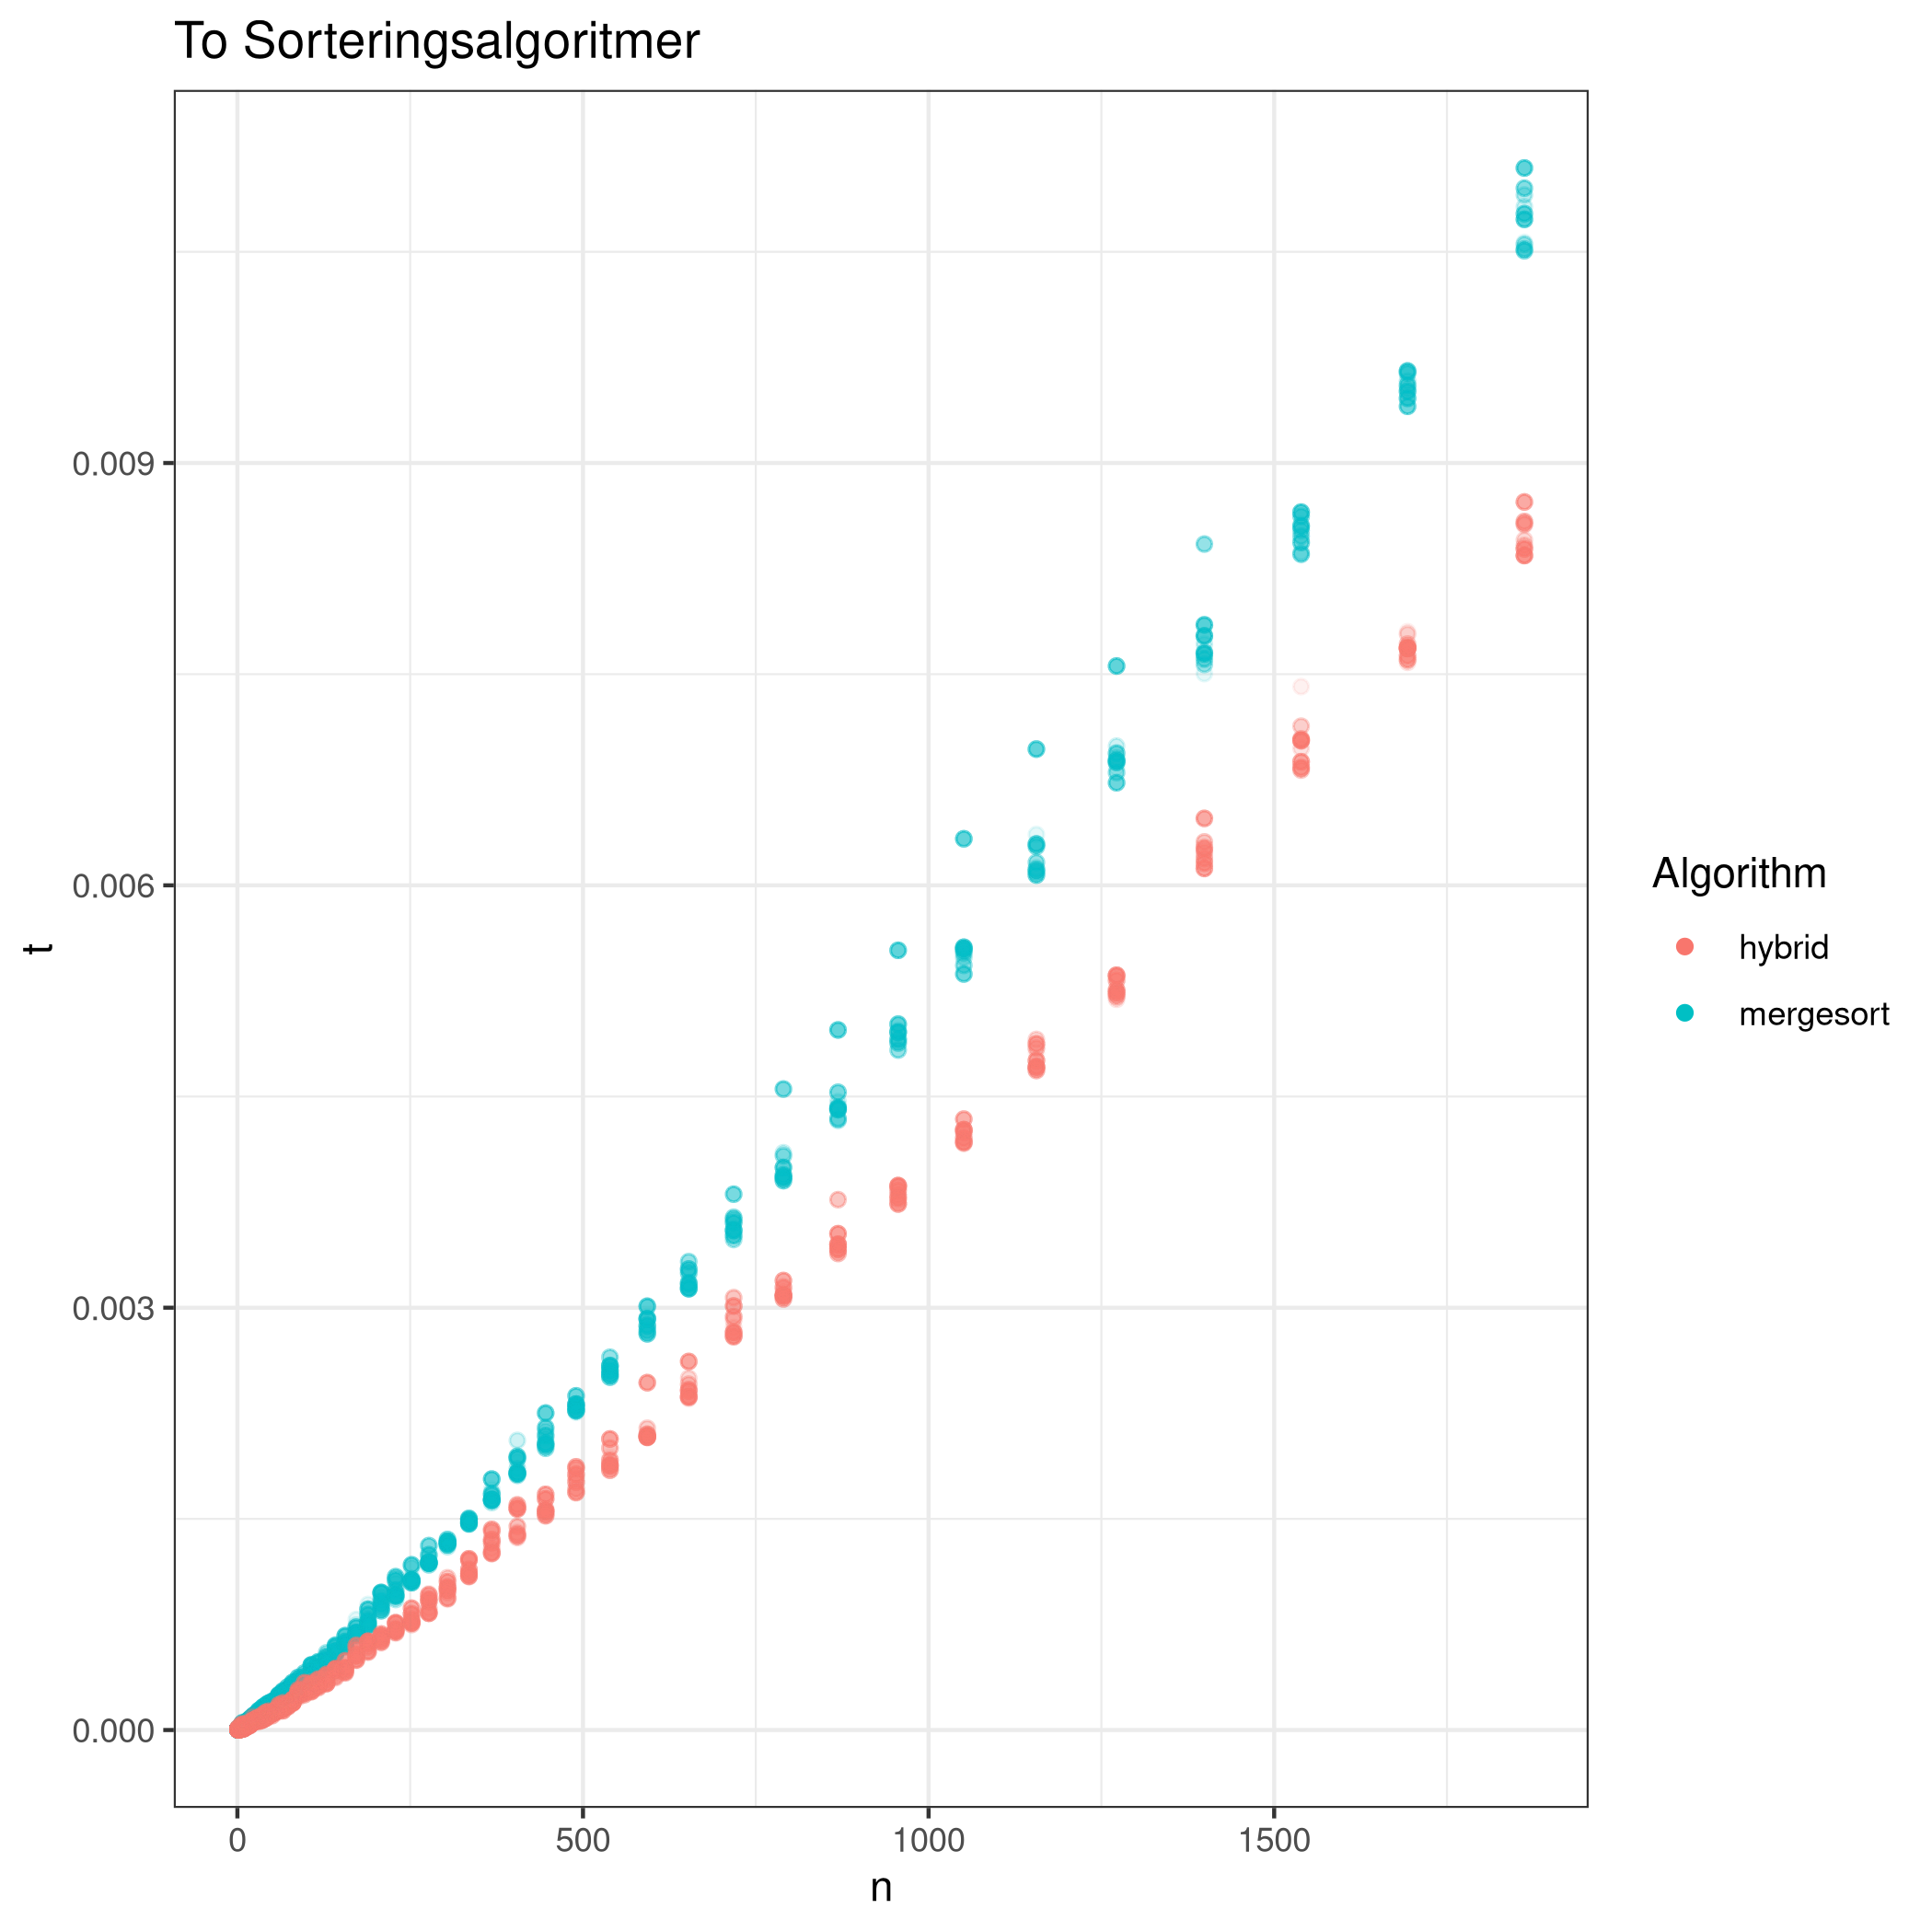
\includegraphics[width=0.45\textwidth]{../img/toMergesort.png}
		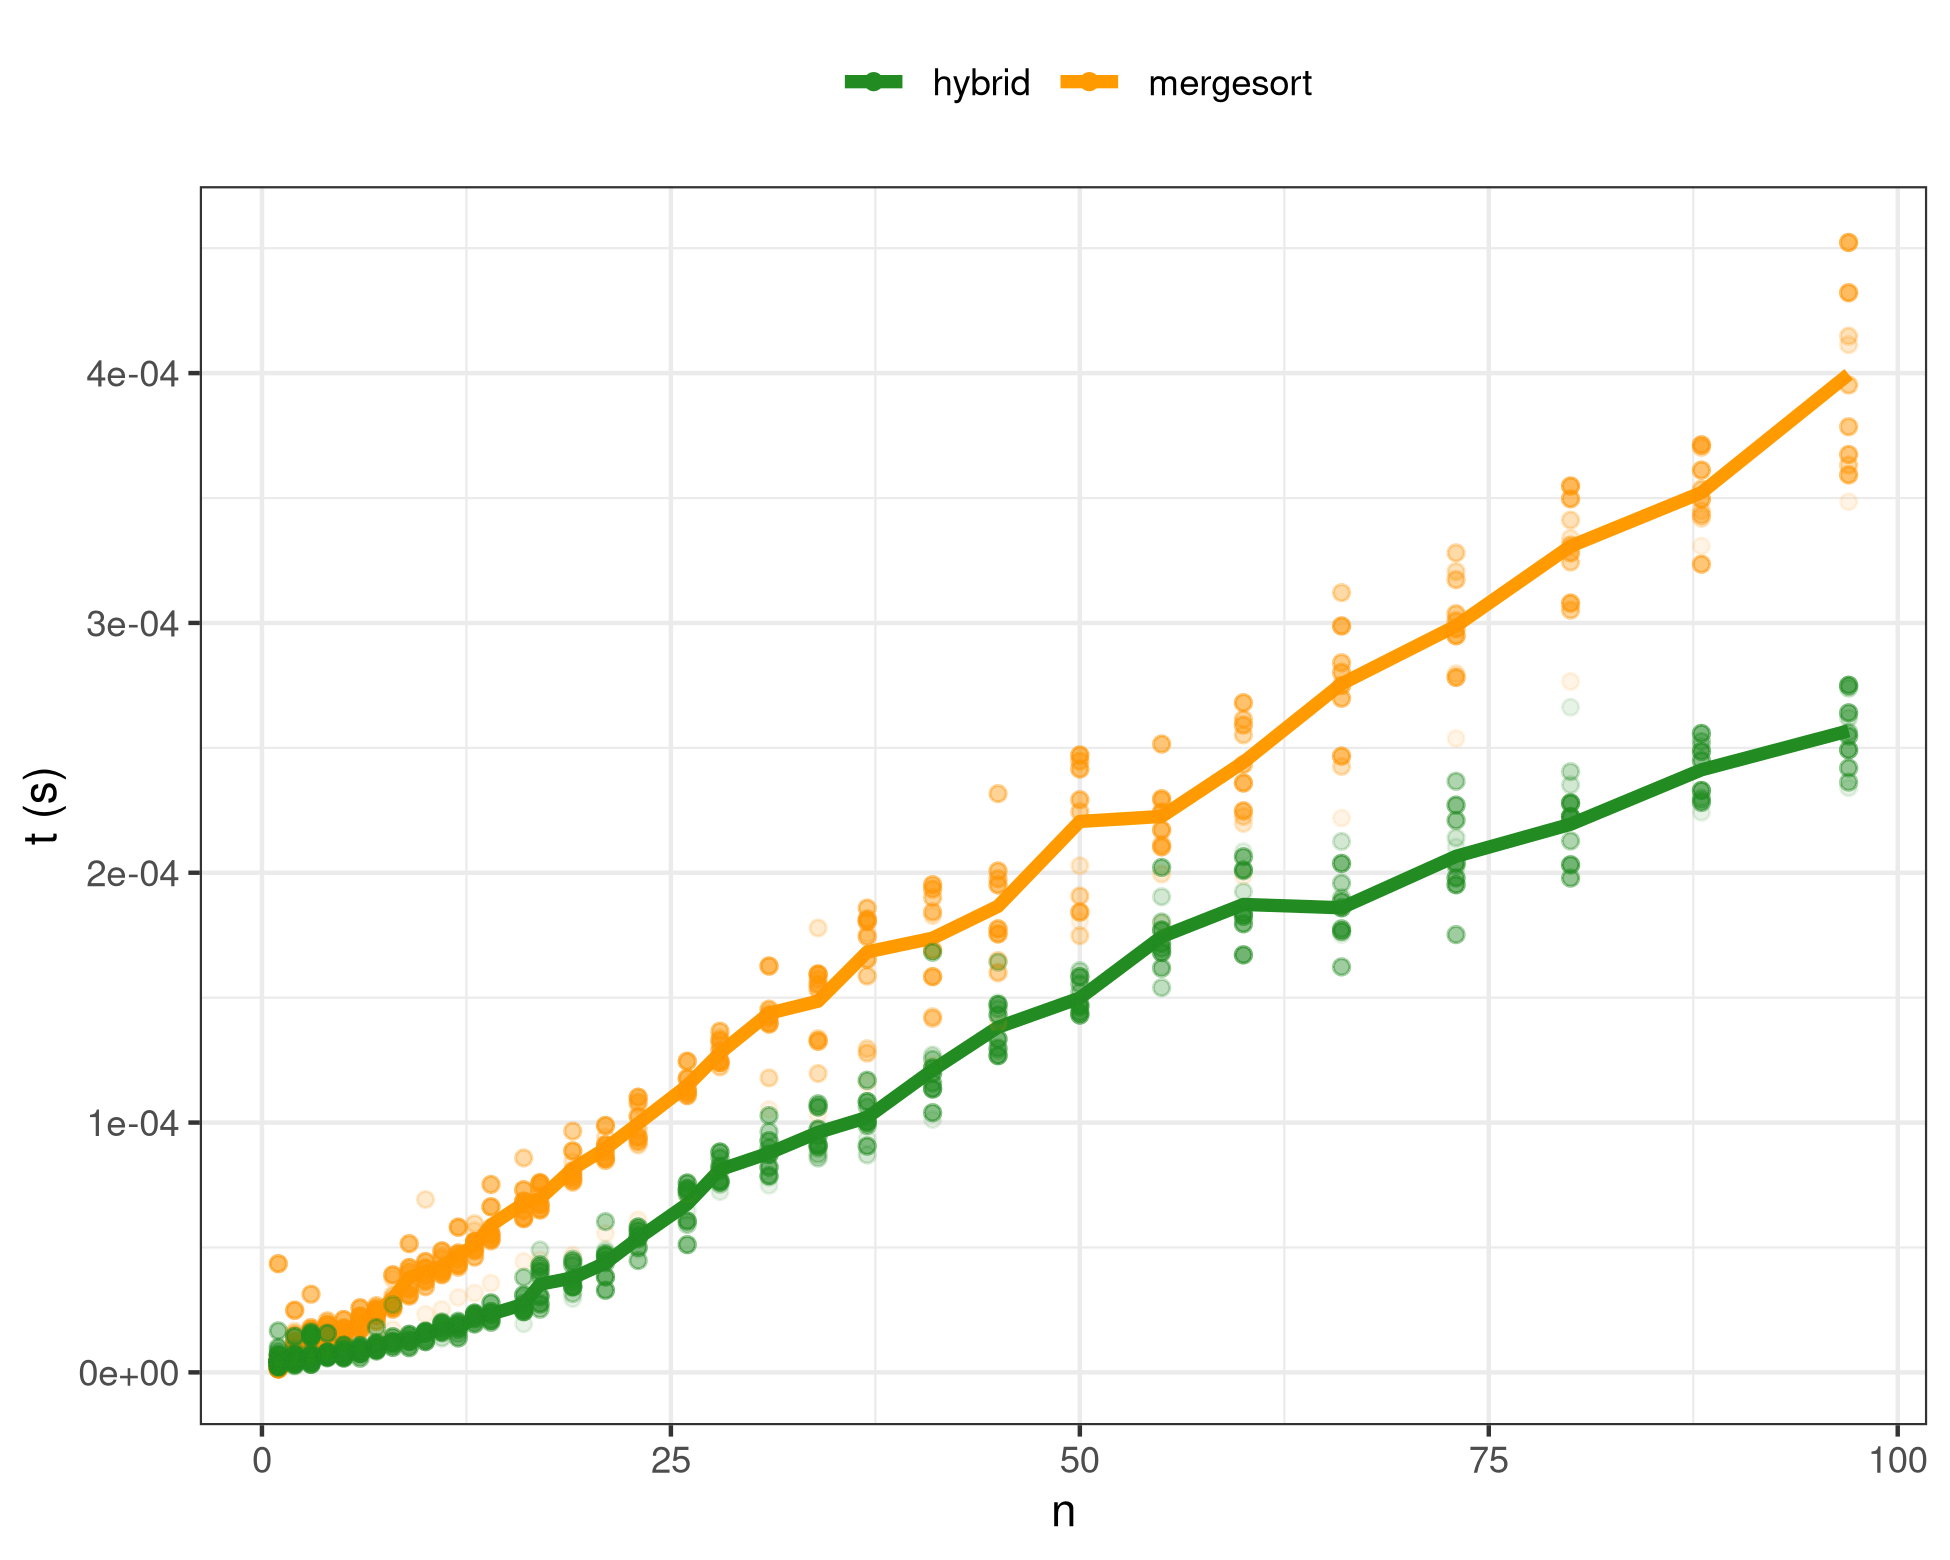
\includegraphics[width=0.45\textwidth]{../img/toMergesortZoomed.png}
		%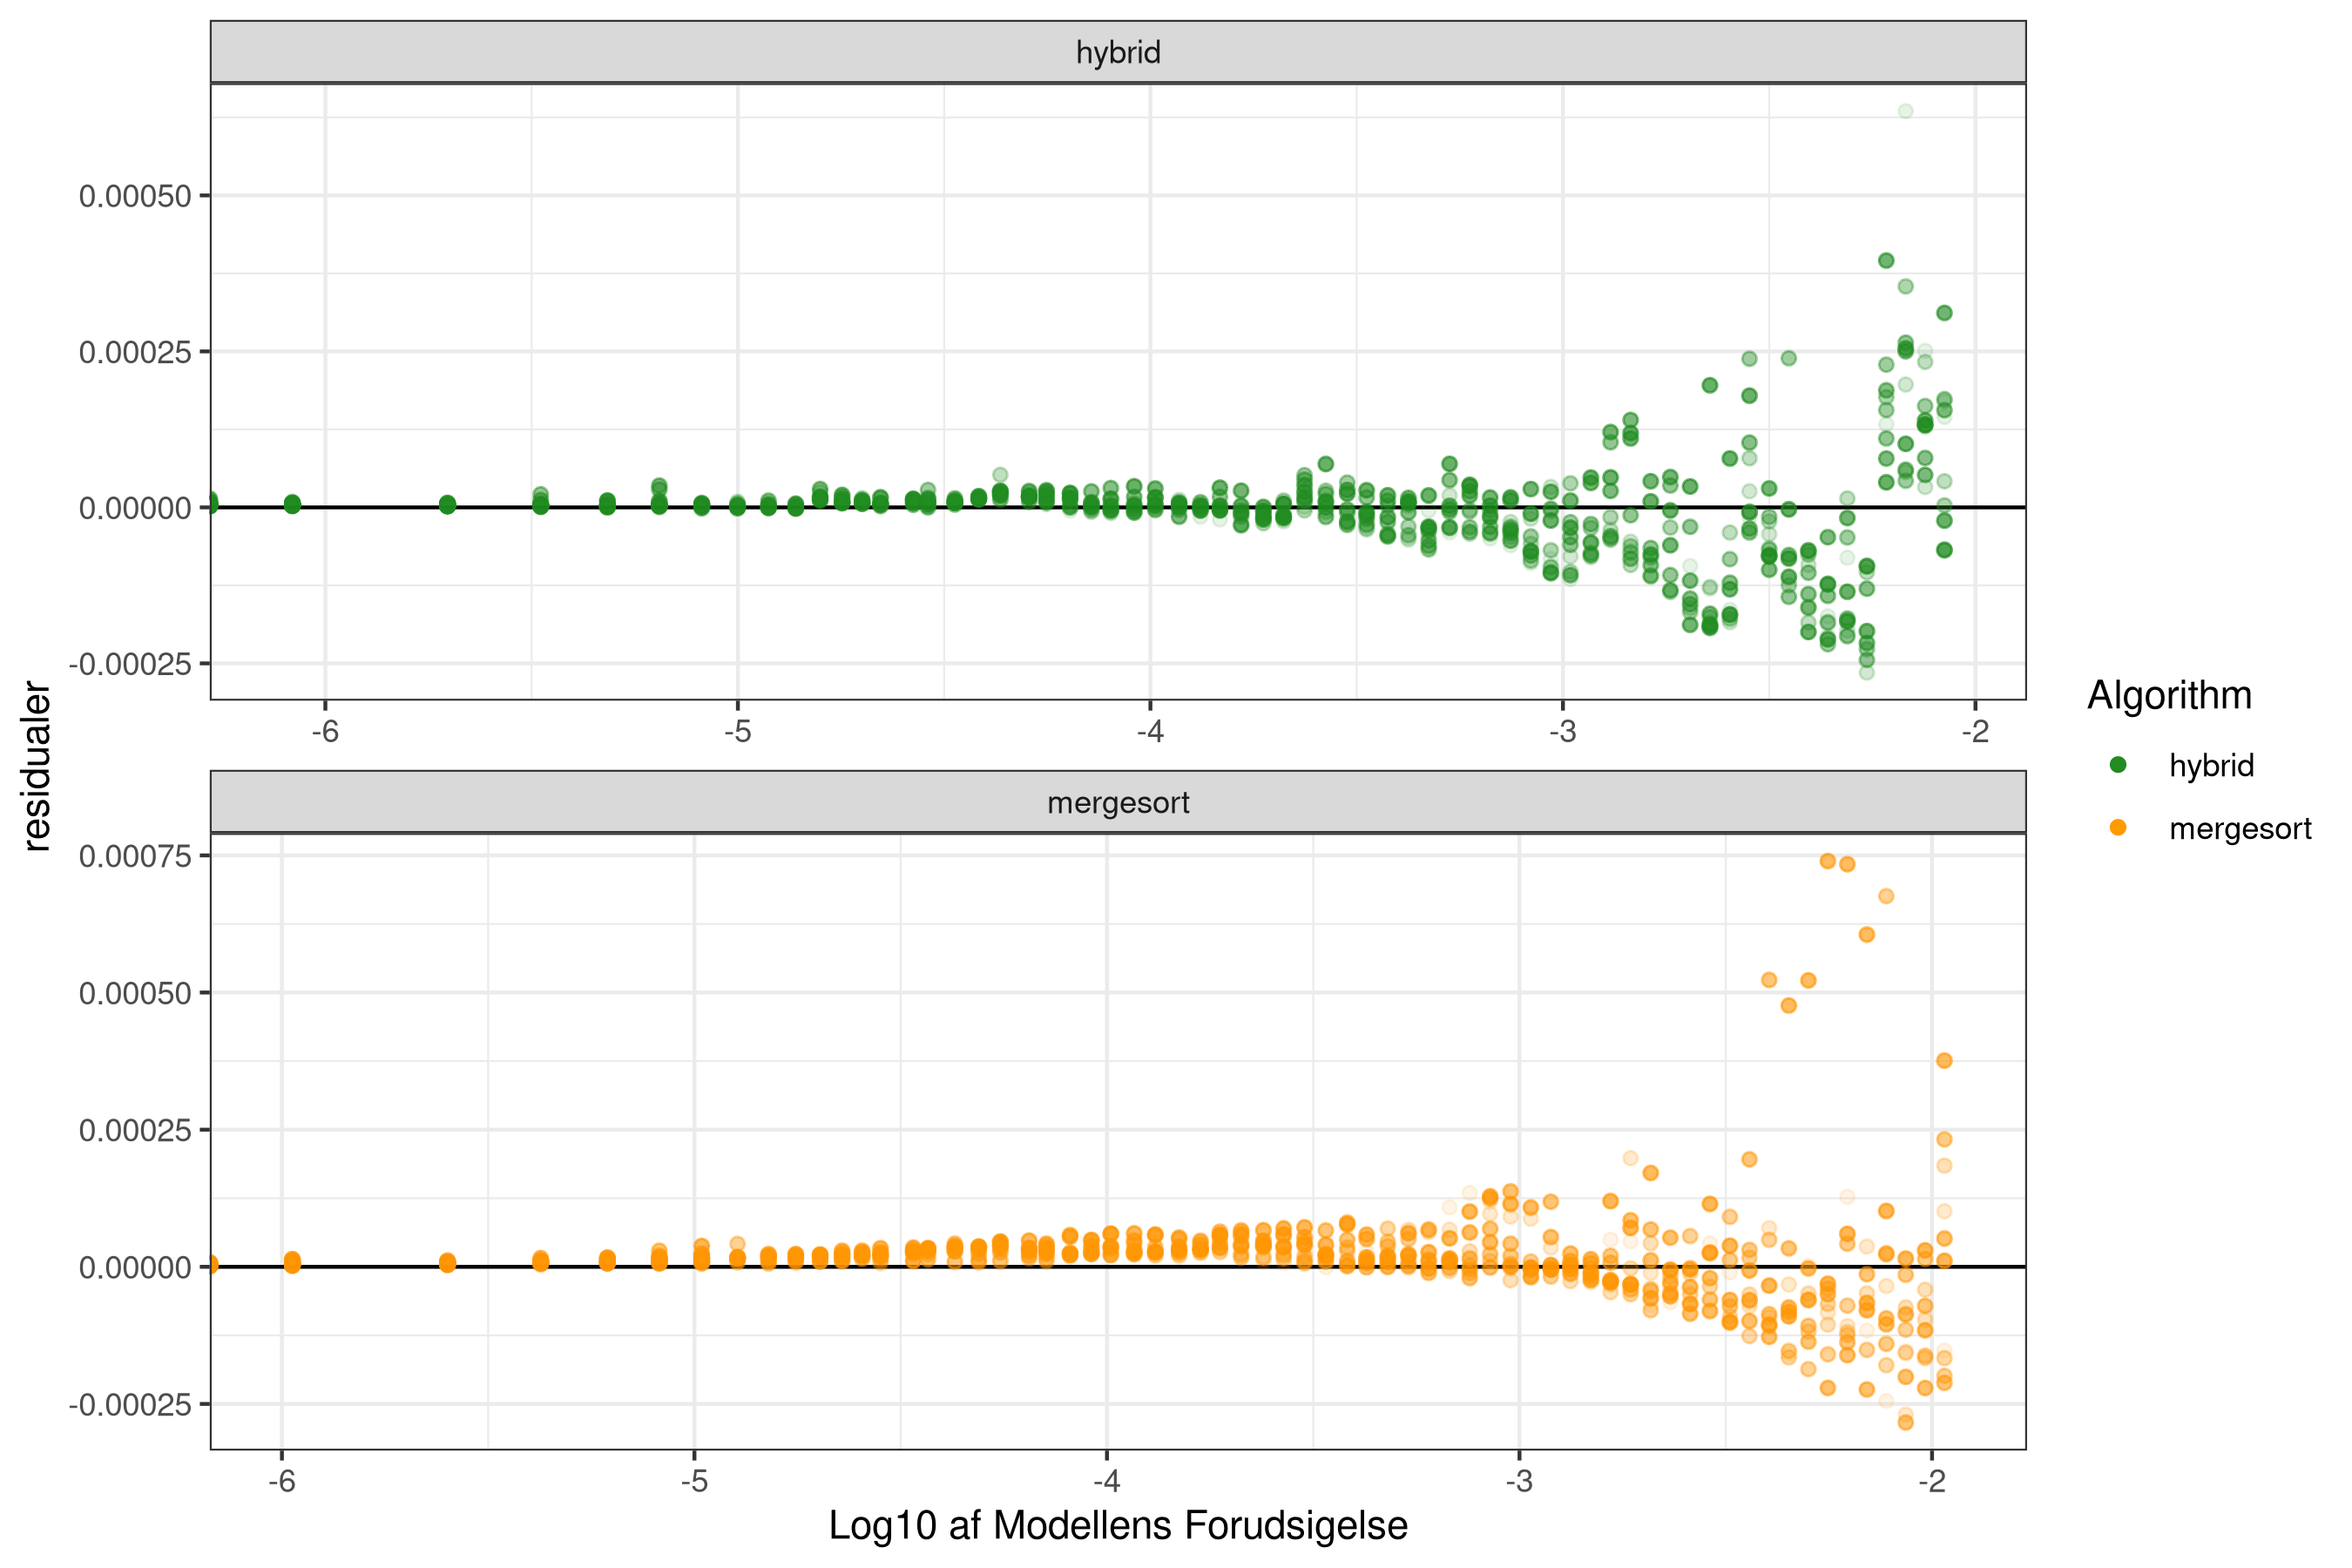
\includegraphics[width=0.45\textwidth]{../img/toMergesortResidual.png}
	\end{center}
	\caption{Reelle udførelsestider for mergesort og hybridalgoritme. Plottet til højre er samme plot som til venste bare zoomet ind, og med en linje der gør mellem gennemsnitet af $t$ for hver $n$}
	\label{fig:Mergesort og Hybridalgoritme}
\end{figure}

